\label {sec:fs-optimization-experiments}

For our experiments, we used the query described in Section \ref{sec:fs-optimization-problem-statement} and the Apache Beam implementation of the NEXMark benchmark model. First, we execute this query using the graph in which \texttt{Auction} and \texttt{Person} are joined first, and the result is joined with \texttt{Bid} (referred to as \textit{Plan 1} in further text); then, we use the graph in which \texttt{Person} and \texttt{Bid} are joined first (\textit{Plan 2}). For each run, we use a different $|Person|:|Auction|:|Bid|$ ratio. To evaluate performance, we measure latency and throughput for each window. We have conducted our experiments on a local machine equipped with a 1.4 GHz Intel Core i5-8257U CPU (4 cores) and 8 GB of memory using the Apache Flink runner. 

Figures \ref{fig:latency_ratio} demonstrates how the latency changes as the $|Person|:|Auction|:|Bid|$ ratio changes. As expected, the plan in which \texttt{Person} and \texttt{Auction} are joined first delivers better results when the arrival rate of \texttt{Bid} records significantly overwhelms the rates of \texttt{Person} and \texttt{Auction}, while the plan in which \texttt{Person} and \texttt{Bid} are joined first works best for cases where the rate of \texttt{Auction} records far exceeds those of \texttt{Person} and \texttt{Bid}. 

Throughput estimation reports similar results, with Plan 1 delivering higher throughput in case of the arrival rate of \texttt{Auction} significantly exceeding that of \texttt{Person} and \texttt{Bid} and Plan 2 performing better in case of the arrival rate of \texttt{Bid} being significantly higher.

\begin{figure}[htbp]
  \centering
  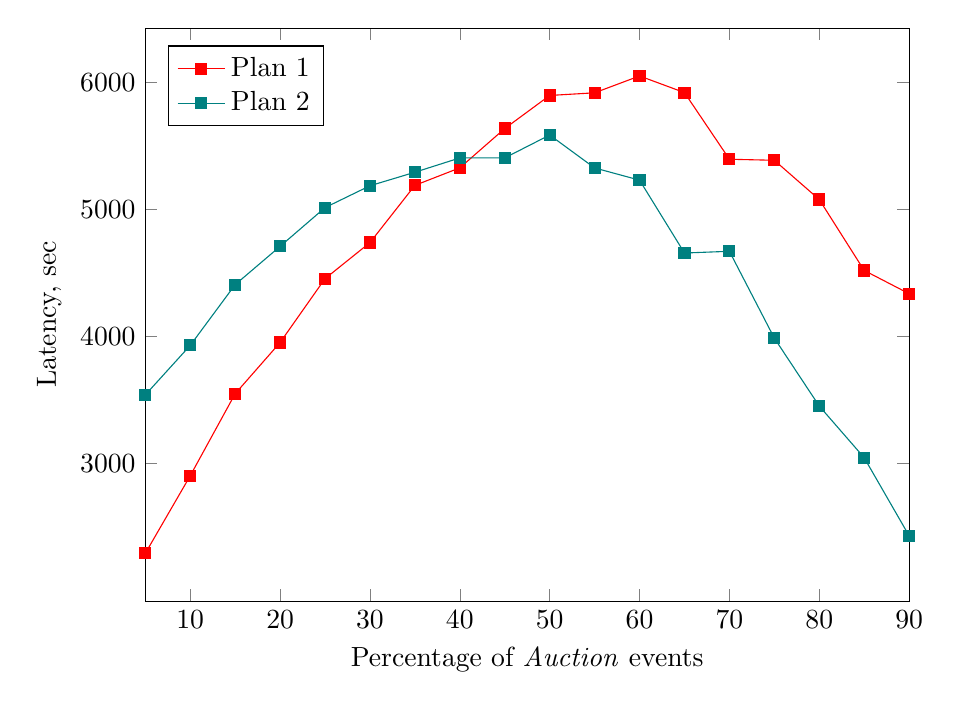
\begin{tikzpicture}
\begin{axis}[
    scale only axis=true,
    width=0.8\textwidth,
    height=0.6\textwidth,
    ytick={3000, 4000, 5000, 6000},
    yticklabels={3000, 4000, 5000, 6000},
    xmin=5, xmax=90,
    legend cell align=left,
    legend pos=north west,
    xlabel={Percentage of \textit{Auction} events},
    ylabel={Latency, sec},
    % x label style={at={(axis description cs:0.5,0.05)},anchor=north},
    % y label style={at={(axis description cs:0.125,0.5)},anchor=center},
]
\addplot[red,mark=square*,mark options={scale=1,solid}] coordinates {
    (5, 2294.73)
    (10, 2905.51)
    (15, 3550.93)
    (20, 3953.99)
    (25, 4456.47)
    (30, 4740.31)
    (35, 5190.68)
    (40, 5328.49)
    (45, 5637.89)
    (50, 5898.18)
    (55, 5918.89)
    (60, 6051.56)
    (65, 5920.56)
    (70, 5396.14)
    (75, 5387.98)
    (80, 5079.04)
    (85, 4520.84)
    (90, 4338.02)
};
\addplot[teal,mark=square*,mark options={scale=1,solid}] coordinates {
    (5, 3541.78)
    (10, 3931.32)
    (15, 4409.38)
    (20, 4710.69)
    (25, 5015.49)
    (30, 5187.45)
    (35, 5293.89)
    (40, 5406.6)
    (45, 5406.6)
    (50, 5586.84)
    (55, 5327.64)
    (60, 5231.65)
    (65, 4658.23)
    (70, 4671.75)
    (75, 3988.29)
    (80, 3453.75)
    (85, 3047.15)
    (90, 2432.85)
};
\legend{
    Plan 1\\
    Plan 2\\
}
\end{axis}
\end{tikzpicture}
  \captionsetup{justification=justified}
  \caption{Latency for different ratios: out of 100 events, $|Person| = 5$, $|Auction|$ is the value on the $x$-axis, $|Bid| = 100 - |Person| - |Auction|$}
  \label {fig:latency_ratio}
\end{figure}

% \begin{figure}[t!]
%     \begin{subfigure}[b]{0.32\textwidth}
%             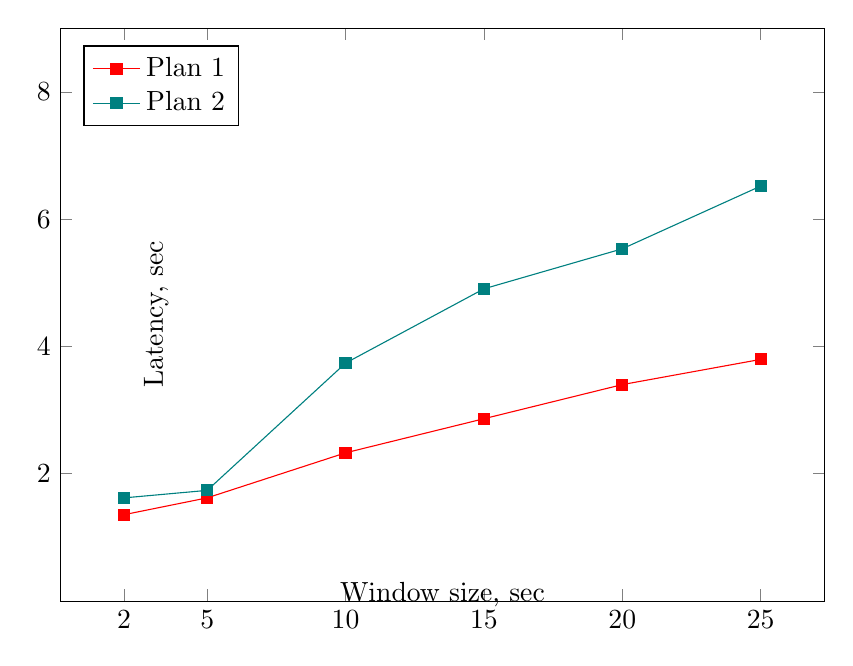
\begin{tikzpicture}
\begin{axis}[
    scale only axis=true,
    width=0.8\textwidth,
    height=0.6\textwidth,
    ymin = 0,
    ymax = 9000,
    ytick={2000, 4000, 6000, 8000},
    yticklabels={2, 4, 6, 8},
    xtick={2, 5, 10, 15, 20, 25},
    xticklabels={$2$, $5$, $10$, $15$, $20$, $25$},
    legend cell align=left,
    legend pos=north west,
    xlabel={Window size, sec},
    ylabel={Latency, sec},
    x label style={at={(axis description cs:0.5,0.05)},anchor=north},
    y label style={at={(axis description cs:0.125,0.5)},anchor=center},
]
\addplot[red,mark=square*,mark options={scale=1,solid}] coordinates {
(2,1357.67)
(5,1621.52)
(10,2328.99)
(15,2864.79)
(20,3400.97)
(25,3796.8)
};
\addplot[teal,mark=square*,mark options={scale=1,solid}] coordinates {
(2,1621.52)
(5,1739.10)
(10,3738.63)
(15,4905.88)
(20,5534.47)
(25,6519.64)
};
\legend{
    Plan 1\\
    Plan 2\\
}
\end{axis}
\end{tikzpicture}
%             \captionsetup{justification=justified}
%             \caption{$|Person|:|Auction|:|Bid|$ = 5:5:90}
%             \label{fig:latency_window_5590}
%     \end{subfigure}
%     % \hspace{2mm}
%     \begin{subfigure}[b]{0.32\textwidth}
%             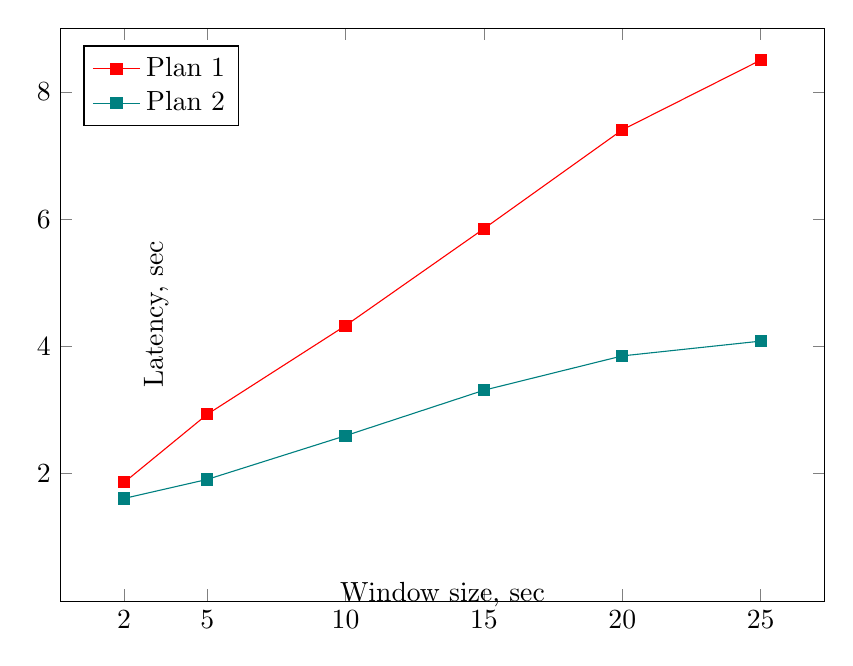
\begin{tikzpicture}
\begin{axis}[
    scale only axis=true,
    width=0.8\textwidth,
    height=0.6\textwidth,
    ymin = 0,
    ymax = 9000,
    ytick={2000, 4000, 6000, 8000},
    yticklabels={2, 4, 6, 8},
    xtick={2, 5, 10, 15, 20, 25},
    xticklabels={$2$, $5$, $10$, $15$, $20$, $25$},
    legend cell align=left,
    legend pos=north west,
    xlabel={Window size, sec},
    ylabel={Latency, sec},
    x label style={at={(axis description cs:0.5,0.05)},anchor=north},
    y label style={at={(axis description cs:0.125,0.5)},anchor=center},
]
\addplot[red, mark=square*, mark options={scale=1,solid}] coordinates {
(2,1864.23)
(5,2933.28)
(10,4327.74)
(15,5850.70)
(20,7403.71)
(25,8498.8)
};
\addplot[teal, mark=square*, mark options={scale=1,solid}] coordinates {
(2,1612.74)
(5,1911.15)
(10,2598.16)
(15,3312.47)
(20,3851.92)
(25,4083.96)
};
\legend{
    Plan 1\\
    Plan 2\\
}
\end{axis}
\end{tikzpicture}
%             \captionsetup{justification=justified}
%             \caption{$|Person|:|Auction|:|Bid|$ = 5:90:5}
%             \label{fig:latency_window_5905}
%     \end{subfigure}
%     \hspace{2mm}
%     \begin{subfigure}[b]{0.32\textwidth}
%             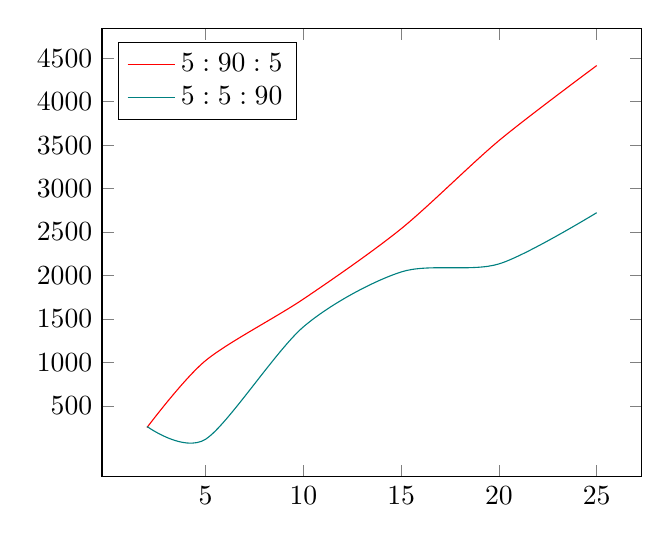
\begin{tikzpicture}
\begin{axis}[
    ytick={500, 1000, 1500, 2000, 2500, 3000, 3500, 4000, 4500},
    yticklabels={$500$, $1000$, $1500$, $2000$, $2500$, $3000$, $3500$, $4000$, $4500$},
    xtick={5, 10, 15, 20, 25},
    xticklabels={$5$, $10$, $15$, $20$, $25$},
    legend cell align=left,
    legend pos=north west
]
\addplot[smooth, red] coordinates {
(2,251.49)
(5,1022.13)
(10,1729.58)
(15,2538.23)
(20,3551.79)
(25,4414.84)
};
\addplot[smooth, teal] coordinates {
(2,263.85)
(5,117.58)
(10,1409.64)
(15,2041.09)
(20,2133.5)
(25,2722.84)
};
\legend{
    $5:90:5$\\
    $5:5:90$\\
}
\end{axis}
\end{tikzpicture}
%             \captionsetup{justification=justified}
%             \caption{Latency difference for Plans 1 and 2}
%             \label{fig:latency_diff_against_window_size}
%     \end{subfigure}
%     \caption{Latency for different window sizes and $|Person|:|Auction|:|Bid|$ ratios}
%     \label{fig:latency_plots}
% \end{figure}

% \begin{figure*}[t!]
%     \begin{subfigure}[b]{0.32\textwidth}
%             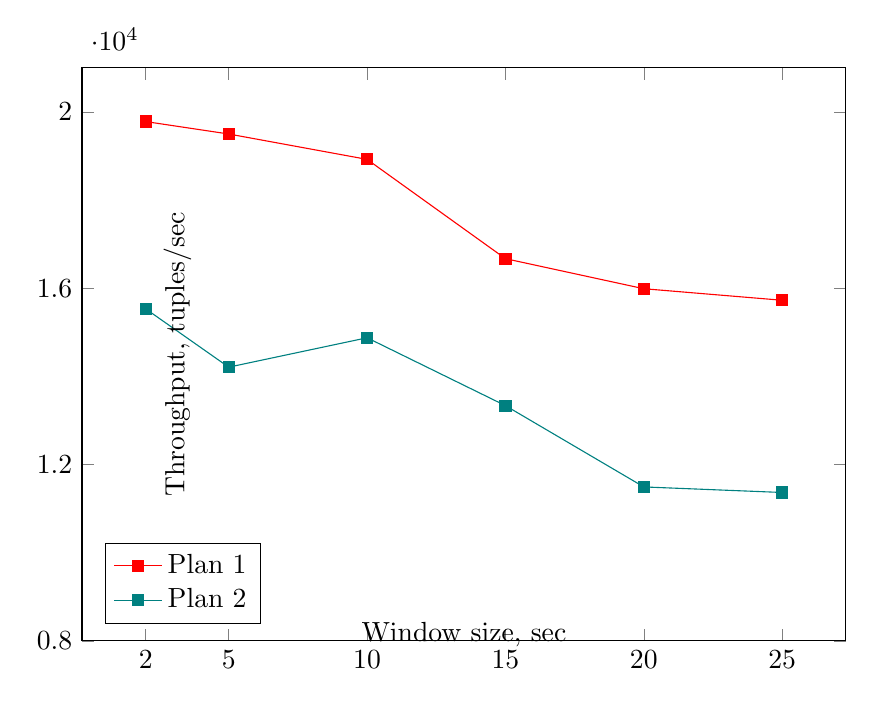
\begin{tikzpicture}
\begin{axis}[
    scale only axis=true,
    width=0.8\textwidth,
    height=0.6\textwidth,
    ymin = 8000,
    ymax = 21000,
    ytick={8000, 12000, 16000, 20000},
    %yticklabels={2, 4, 6, 8},
    xtick={2, 5, 10, 15, 20, 25},
    xticklabels={$2$, $5$, $10$, $15$, $20$, $25$},
    legend cell align=left,
    legend pos=south west,
    xlabel={Window size, sec},
    ylabel={Throughput, tuples/sec},
    x label style={at={(axis description cs:0.5,0.05)},anchor=north},
    y label style={at={(axis description cs:0.125,0.5)},anchor=center},
]
\addplot[red, mark=square*, mark options={scale=1,solid}] coordinates {
(2,19782.8)
(5,19500.8)
(10,18924.7)
(15,16671.4)
(20,15989.5)
(25,15727.7)
};
\addplot[teal, mark=square*, mark options={scale=1,solid}] coordinates {
(2,15532.8)
(5,14209.6)
(10,14876.5)
(15,13336.4)
(20,11491.7)
(25,11365.6)
};
\legend{
    Plan 1\\
    Plan 2\\
}
\end{axis}
\end{tikzpicture}
%             \captionsetup{justification=justified}
%             \caption{$|Person|:|Auction|:|Bid|$ = 5:5:90}
%             \label{fig:throughput_window_5590}
%     \end{subfigure}
%     \hspace{2mm}
%     \begin{subfigure}[b]{0.32\textwidth}
%             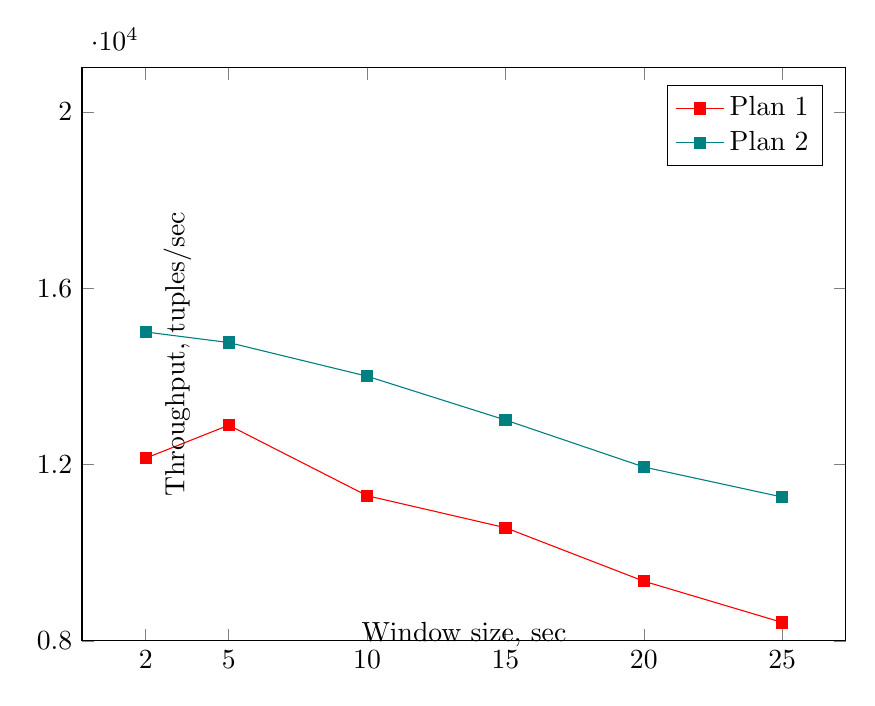
\begin{tikzpicture}
\begin{axis}[
    scale only axis=true,
    width=0.8\textwidth,
    height=0.6\textwidth,
    ymin = 8000,
    ymax = 21000,
    ytick={8000, 12000, 16000, 20000},
    %yticklabels={2, 4, 6, 8},
    xtick={2, 5, 10, 15, 20, 25},
    xticklabels={$2$, $5$, $10$, $15$, $20$, $25$},
    legend cell align=left,
    legend pos=north east,
    xlabel={Window size, sec},
    ylabel={Throughput, tuples/sec},
    x label style={at={(axis description cs:0.5,0.05)},anchor=north},
    y label style={at={(axis description cs:0.125,0.5)},anchor=center},
]
\addplot[red, mark=square*, mark options={scale=1,solid}] coordinates {
(2,12144.02)
(5,12892.16)
(10,11292.62)
(15,10566.26)
(20,9352.6)
(25,8416.64)
};
\addplot[teal, mark=square*, mark options={scale=1,solid}] coordinates {
(2,15007.76)
(5,14768.28)
(10,14004.28)
(15,13010.24)
(20,11943.94)
(25,11262.62)
};
\legend{
    Plan 1\\
    Plan 2\\
}
\end{axis}
\end{tikzpicture}
%             \captionsetup{justification=justified}
%             \caption{$|Person|:|Auction|:|Bid|$ = 5:90:5}
%             \label{fig:throughput_window_5905}
%     \end{subfigure}
%     \hspace{2mm}
%     \begin{subfigure}[b]{0.32\textwidth}
%             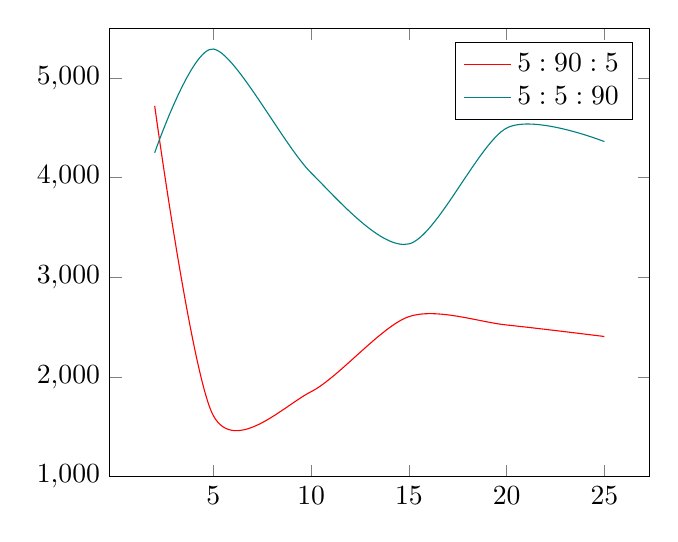
\begin{tikzpicture}
\begin{axis}[
    ymin=1000, ymax=5500,
    xtick={5, 10, 15, 20, 25},
    xticklabels={$5$, $10$, $15$, $20$, $25$},
    legend cell align=left,
    legend pos=north east
]
\addplot[smooth, red] coordinates {
(2,4721.1)
(5,1611.0)
(10,1851.7)
(15,2604.9)
(20,2521.2)
(25,2405.5)
};
\addplot[smooth, teal] coordinates {
(2,4250.0)
(5,5291.2)
(10,4048.2)
(15,3335)
(20,4497.8)
(25,4362.1)
};
\legend{
    $5:90:5$\\
    $5:5:90$\\
}
\end{axis}
\end{tikzpicture}
%             \captionsetup{justification=justified}
%             \caption{Throughput difference for Plans 1 and 2}
%             \label{fig:throughput_diff_against_window_size}
%     \end{subfigure}
%     \caption{Throughput for different window sizes and $|Person|:|Auction|:|Bid|$ ratios}
%     \label{fig:throughput_plots}
% \end{figure*}


The results of our experiments demonstrate that streaming query execution performance depends on the plan used for the execution, and the optimality of the plan depends on the data characteristics, which proves the necessity of adaptive optimization of streaming queries. The first steps towards adaptive optimization should be predicting statistics for each window and performing runtime graph migration, since the results of the experiments show that even the current planners could use those statistics to produce a better execution plan. These two challenges will be the focus of our future work.

